\subsection{Sample Application of Formal and Insight Model}

\begin{figure}[!htbp]
    \centering
    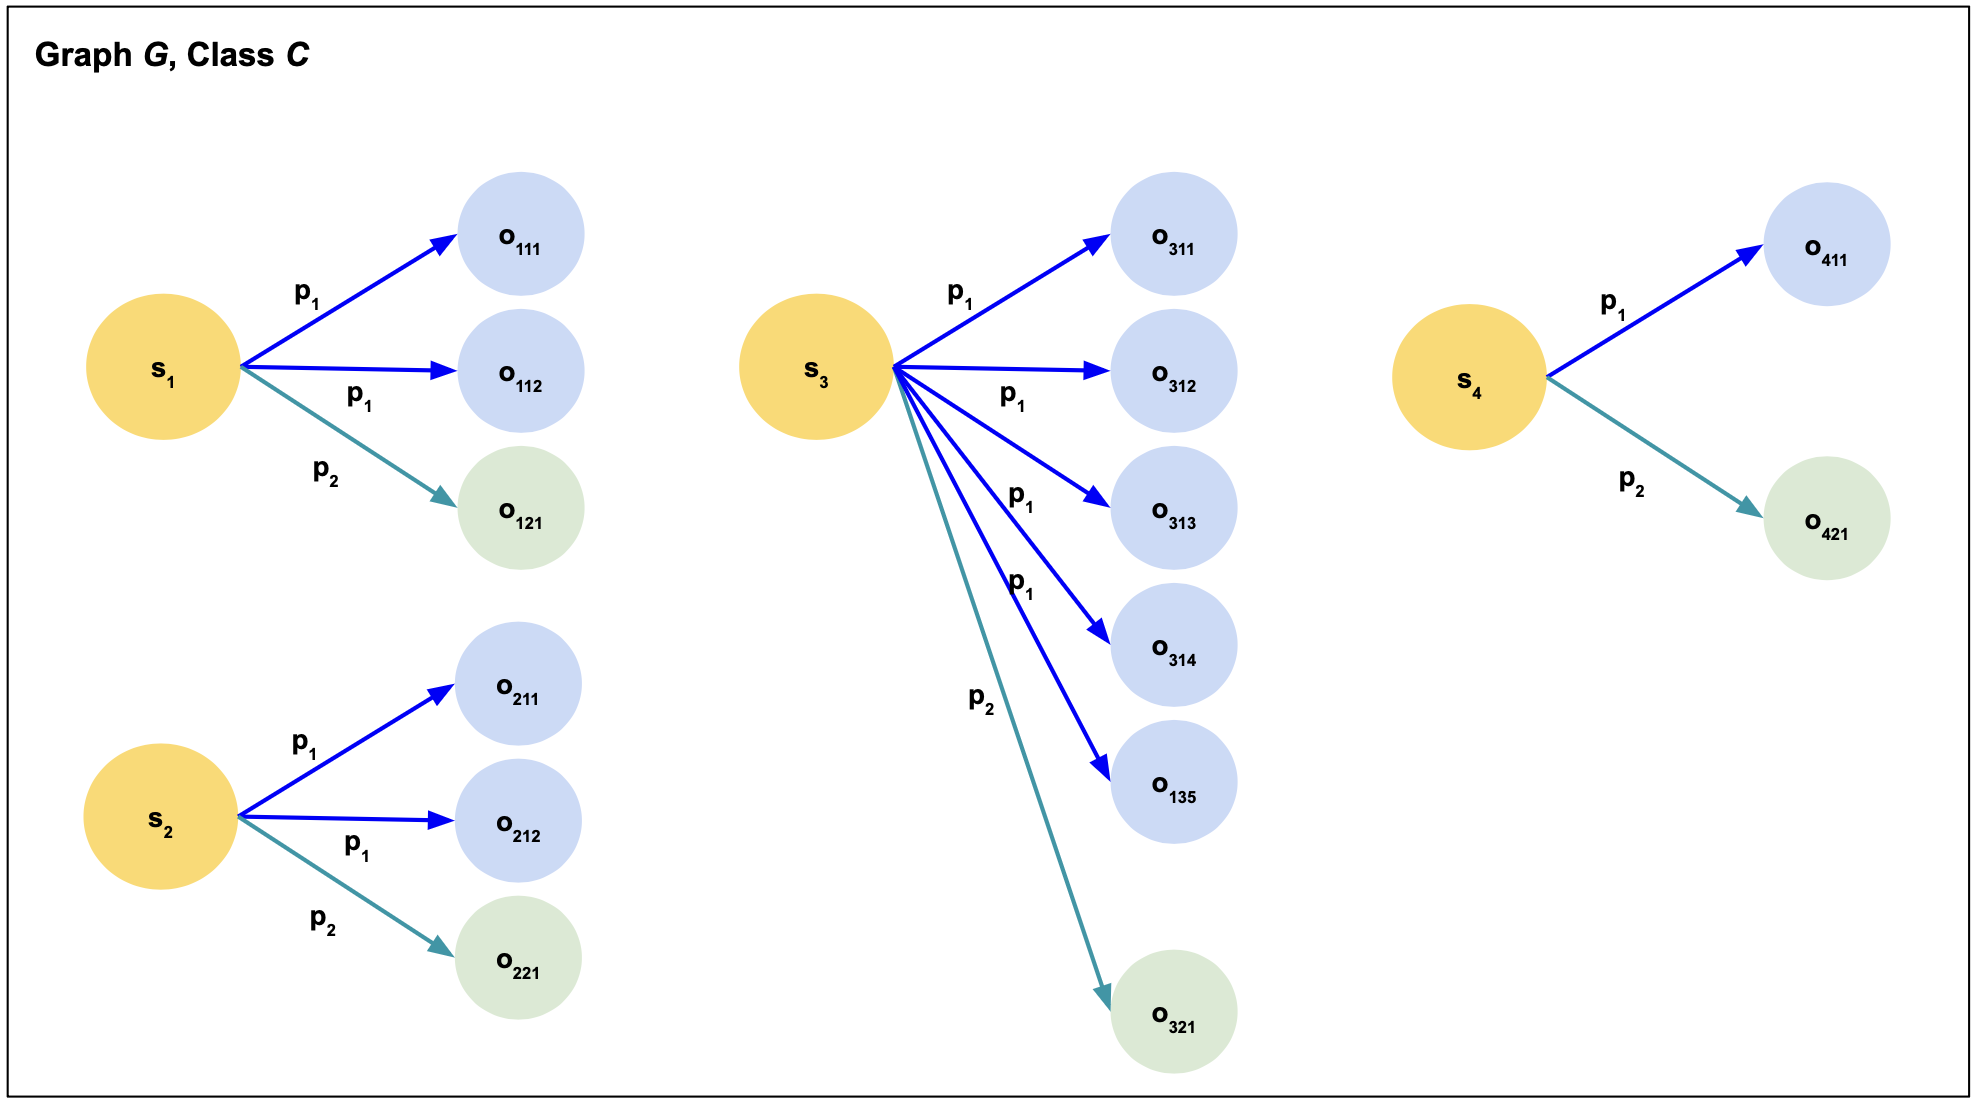
\includegraphics[scale=.4]{Wealth Weighted}
    \caption{Sample knowledge graph \(G\) that contains class \(C\) with 4 entities (\(s_1\)-\(s_4\)), represented as yellow nodes (subjects in RDF triples). Edges represent properties: blue edges correspond to property \(p_1\) and green edges to property \(p_2\). Object nodes are color-coded to match their associated property: blue circles indicate objects linked via \(p_1\), and green circles indicate objects linked via \(p2\).} \label{fig:wealth-weighted}
\end{figure}

We provide small case in \autoref{fig:wealth-weighted} to illustrate how both models can be applied in quantifying knowledge wealth. In this example, we will focus on the notion using bag of properties with outgoing direction of link to quantify the wealth.

A graph \(G\) has a class \(C\), which consists of four entities \(s_1\), \(s_2\), \(s_3\), and \(s_4\). Each entity has two distinct properties \(p_1\) and \(p_2\). For example, entity \(s_1\) is linked by property \(p_1\) to objects \(o_{111}\) and \(o_{112}\), and by property \(p_2\) to object \(o_{121}\). Using the bag of properties and outgoing link direction, the wealth of entity \(s_1\) is 3 (2 accounted for by \(p_1\) and 1 by \(p_2\)). Similarly, the wealth of entities \(s_2\), \(s_3\), and \(s_4\) is 3, 6, and 2, respectively. \autoref{tab:sample statistical summary} provides a statistical summary describing the wealth of class \(C\). Entities in class \(C\) have a mean wealth of 3.5, a median wealth of 3, a mode wealth of 3, a minimum wealth of 2, and a maximum wealth of 6. Based on each individual entity's wealth, the imbalance measure of class \(C\) is quantified using the Gini coefficient, which has a value of 0.21.

\begin{center}
    \scriptsize
    \begin{threeparttable}
    \captionsetup{font=small}
    \caption{Statistical Summary of Wealth of Class \(C\)}
    \label{tab:sample statistical summary}
    \begin{tabular}{c | c c c c c c c} 
    
    \toprule
        Measure & Entity Count & Mean & Median & Mode & Minimum & Maximum & Gini \\ [0.5ex] 
    \midrule
        Value & 4 & 3.5 & 3 & 3 & 2 & 6 & 0.21 \\
        [0.5ex]
    \bottomrule
    \end{tabular}
    \begin{tablenotes}
        \scriptsize
        \item{This table shows some statistical measures to quantify the wealth of class \(C\).}
    \end{tablenotes}
    \end{threeparttable}
\end{center}

\begin{figure}[!htbp]
    \centering
    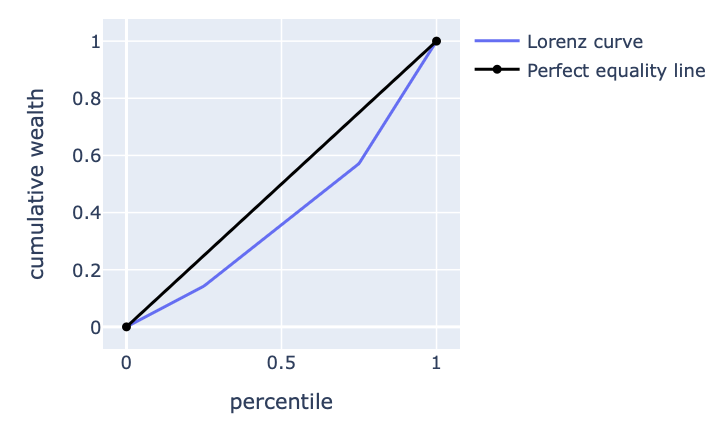
\includegraphics[scale=0.6]{Sample Lorenz Curve}
    \caption{Lorenz curve of class \(C\)} \label{fig:sample-lorenz}
\end{figure}

In addition to the Gini coefficient, the Lorenz curve for the wealth of entities in class \(C\) is shown in \autoref{fig:sample-lorenz}. This figure illustrates that the wealth distribution within class \(C\) is very close to the diagonal line of perfect equality, which aligns with the small Gini coefficient value of 0.21.